% Vygenerováno skriptem vysledky.py z výsledků hodnocení. Čísla odpovídají tabulkám.
% Při změně dat spusťte skript znovu; ruční úpravy tohoto souboru se tím přepíšou.
\section{Výsledky}
\label{sec:vysledky}

Tabulka~\ref{tab:vysledky} a~obrázek~\ref{fig:m1} shrnují výsledky 3~systémů na testovací sadě (10~vět, každá zadaná v~každé podmínce promptu jednou). Hlavní metrika M1 udává podíl vět, u~nichž odpověď obsahovala úplnou a~přesnou množinu podob všech víceznačných slov a~žádnou závorku navíc. S~výchozím promptem (P1) byla M1 mezi 10 a~20~\%, se strukturovaným (P2) mezi 10 a~80~\% a~s~optimalizovaným (P3) mezi 20 a~100~\%. Nejvyšší hodnotu, 100~\%, má Gemini (P3).

Hypotéza předpokládá, že strukturovaný prompt zvýší M1 oproti výchozímu. Na stejných větách se M1 mezi P1 a~P2 zvýšila u~2 z~3 systémů a~nevážený průměr změny je $+$26{,}7~p.~b. (ChatGPT 0, Gemini $+$70, Claude $+$10; tabulka~\ref{tab:efekt-promptu}). Kritérium stanovené v~hypotéze, tedy zlepšení souhrnně i~u~většiny systémů, je v~těchto datech splněno. Optimalizovaný prompt změnil M1 oproti strukturovanému v~průměru o~$+$20~p.~b. (zlepšení u~3 z~3 systémů; ChatGPT $+$10, Gemini $+$20, Claude $+$30).

Nejistotu skóre vyjadřujeme 95\% Wilsonovými intervaly \cite{wilson1927}. Popisují nejistotu danou malým počtem vět, nikoli kolísání odpovědí při opakovaném zadání. Při 10~větách jsou intervaly široké, od 27{,}8 do 51{,}9~p.~b. Nepřekrývají se pouze intervaly těchto dvojic: ChatGPT a~Gemini (P2), ChatGPT a~Gemini (P3). Rozdíly mezi systémy proto uvádíme jako pozorování na této sadě, ne jako doklad obecné převahy některého z~nich.

Každá věta byla v~každé podmínce zadána jednou, analýza opakovaných běhů proto není relevantní. Technická selhání služby se v~hodnocených bězích nevyskytla.

Alternativní vysvětlení říká, že strukturovaný prompt jen zvýší ochotu označovat slova za víceznačná. Odpovědí, v~nichž systém dal do závorky slovo, které víceznačné není, bylo s~P1 1 z~30, s~P2 2 z~30 a~s~P3 0 z~30 (obrázek~\ref{fig:falesne}). Takových odpovědí se strukturovaným promptem přibylo, alternativní vysvětlení proto nelze vyloučit. Odpovědí porušujících formát (víc řádků nebo neplatná závorka) bylo s~P1 6, s~P2 10 a~s~P3 4; počítají se jako chybné.

Porovnání kvality a~úsilí ukazují tabulka~\ref{tab:usili} a~obrázek~\ref{fig:latence}. Výchozí prompt má 763 znaků, strukturovaný 3635 a~optimalizované 3114 až 5504. Ladění optimalizovaného promptu navíc stálo u~každého systému 30 vývojových a~validačních dotazů. Medián doby do prvního textu odpovědi (M3) se mezi P1 a~P3 změnil takto: ChatGPT z~1{,}3 na 1{,}6~s; Gemini z~6{,}5 na 13{,}2~s; Claude z~2{,}1 na 4{,}6~s. Vyšší přesnost optimalizovaného promptu je tedy třeba vážit proti delšímu promptu, času na ladění a~době odezvy; metriky neslučujeme do jednoho skóre.

% Vygenerováno skriptem vysledky.py — neupravujte ručně, raději skript spusťte znovu.
% Vyžaduje balíčky booktabs a tabularx (v mereni.tex už jsou).

\begin{table}[htbp]
\centering\small
\caption{Výsledky na testovací sadě: M1 (úplná a přesná množina podob), M2 (správnost zbytku věty), odpovědi s falešně označenou víceznačností, odpovědi porušující formát (víc řádků nebo neplatná závorka; počítají se jako chybné v~M1 i~M2) a M3 (medián doby do prvního textu). IS jsou 95\% Wilsonovy intervaly; popisují nejistotu mezi úlohami, ne variabilitu opakovaného generování.}
\label{tab:vysledky}
\begin{tabular}{@{}llcccccc@{}}
\toprule
Systém & Prompt & M1 & M1 95\% IS & M2 & Falešná víc. & Formát & M3 medián [Q1--Q3] \\
 & & (úloh) & (\%) & (úloh) & (odpovědí) & (chybných) & (s) \\
\midrule
ChatGPT & P1 & 1/10 & 1{,}8--40{,}4 & 7/10 & 0/10 & 2/10 & 1{,}3 [1{,}1--1{,}5] \\
 & P2 & 1/10 & 1{,}8--40{,}4 & 6/10 & 1/10 & 3/10 & 1{,}2 [1{,}1--1{,}3] \\
 & P3 & 2/10 & 5{,}7--51{,}0 & 7/10 & 0/10 & 3/10 & 1{,}6 [1{,}5--1{,}7] \\
\addlinespace
Gemini & P1 & 1/10 & 1{,}8--40{,}4 & 9/10 & 1/10 & 0/10 & 6{,}5 [2{,}4--7{,}5] \\
 & P2 & 8/10 & 49{,}0--94{,}3 & 9/10 & 0/10 & 1/10 & 12{,}9 [9{,}1--18{,}5] \\
 & P3 & 10/10 & 72{,}2--100{,}0 & 10/10 & 0/10 & 0/10 & 13{,}2 [9{,}8--25{,}3] \\
\addlinespace
Claude & P1 & 2/10 & 5{,}7--51{,}0 & 6/10 & 0/10 & 4/10 & 2{,}1 [1{,}6--3{,}5] \\
 & P2 & 3/10 & 10{,}8--60{,}3 & 3/10 & 1/10 & 6/10 & 2{,}7 [1{,}6--5{,}6] \\
 & P3 & 6/10 & 31{,}3--83{,}2 & 9/10 & 0/10 & 1/10 & 4{,}6 [3{,}2--7{,}0] \\
\bottomrule
\end{tabular}
\end{table}

\begin{table}[htbp]
\centering\small
\caption{Změna M1 mezi podmínkami promptu na stejných úlohách (testovací sada), v~procentních bodech. V~závorce počet úloh, které se zlepšily\,/\,zhoršily. Průměr je nevážený přes systémy; bez testu významnosti.}
\label{tab:efekt-promptu}
\begin{tabular}{@{}lccc@{}}
\toprule
Systém & P1 $\rightarrow$ P2 & P2 $\rightarrow$ P3 & P1 $\rightarrow$ P3 \\
\midrule
ChatGPT & 0 (0\,/\,0) & $+$10 (1\,/\,0) & $+$10 (1\,/\,0) \\
Gemini & $+$70 (7\,/\,0) & $+$20 (2\,/\,0) & $+$90 (9\,/\,0) \\
Claude & $+$10 (3\,/\,2) & $+$30 (3\,/\,0) & $+$40 (4\,/\,0) \\
\midrule
Průměr systémů & $+$27 & $+$20 & $+$47 \\
Zlepšených systémů & 2 z 3 & 3 z 3 & 3 z 3 \\
\bottomrule
\end{tabular}
\end{table}

\begin{table}[htbp]
\centering\small
\caption{Úsilí: označení modelu viditelné v~rozhraní, délka promptu ve znacích bez testované věty a~zmrazená verze optimalizovaného promptu. Ladění P3 navíc u~každého systému stálo 30 vývojových a~validačních dotazů.}
\label{tab:usili}
\begin{tabular}{@{}llrrrc@{}}
\toprule
Systém & Model & P1 & P2 & P3 & Verze P3 \\
\midrule
ChatGPT & GPT-6 Luna & 763 & 3635 & 4583 & v2 \\
Gemini & 3.8 Flash-Lite & 763 & 3635 & 3114 & v5 \\
Claude & Sonnet 5.5 & 763 & 3635 & 5504 & v6 \\
\bottomrule
\end{tabular}
\end{table}

% Vygenerováno skriptem vysledky.py. Vyžaduje \usepackage{graphicx} v preambuli.

\begin{figure}[htbp]
\centering
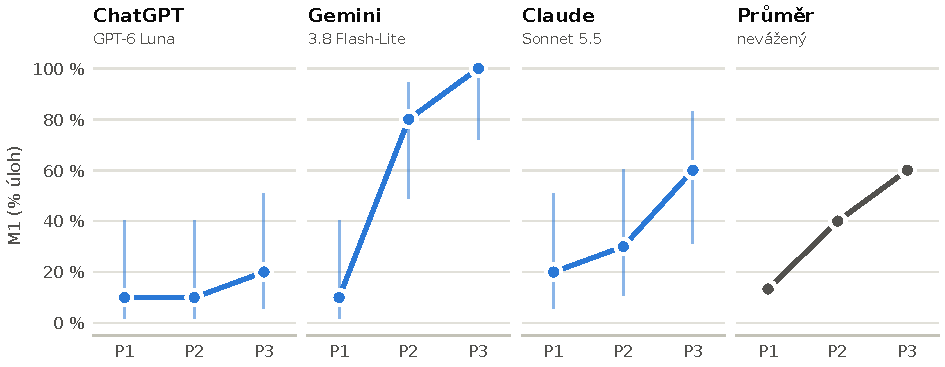
\includegraphics[width=\linewidth]{vystupy/graf_m1.pdf}
\caption{M1 podle systému a~podmínky promptu na testovací sadě. Body jsou podíly úloh s~úplnou a~přesnou množinou podob, svislé úsečky 95\% Wilsonovy intervaly. Průměr systémů je nevážený a~bez intervalu.}
\label{fig:m1}
\end{figure}

\begin{figure}[htbp]
\centering
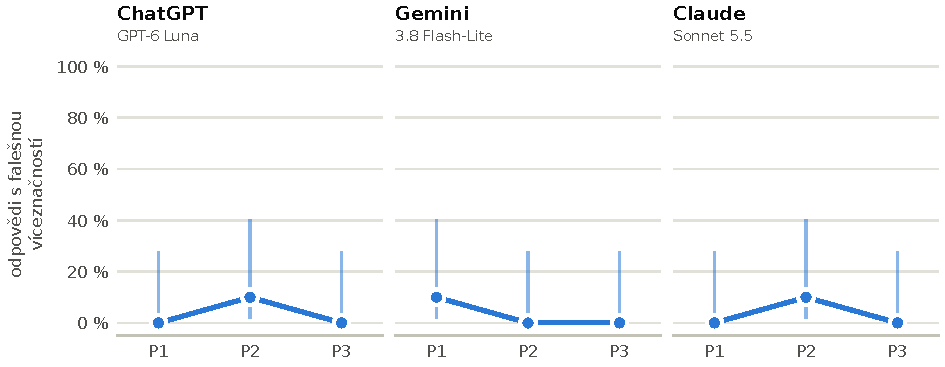
\includegraphics[width=\linewidth]{vystupy/graf_falesne.pdf}
\caption{Podíl odpovědí, v~nichž systém označil za víceznačné slovo, které víceznačné není, s~95\% Wilsonovými intervaly. Odpovědi vyřazené pro chybu formátu se sem nepromítají.}
\label{fig:falesne}
\end{figure}

\begin{figure}[htbp]
\centering
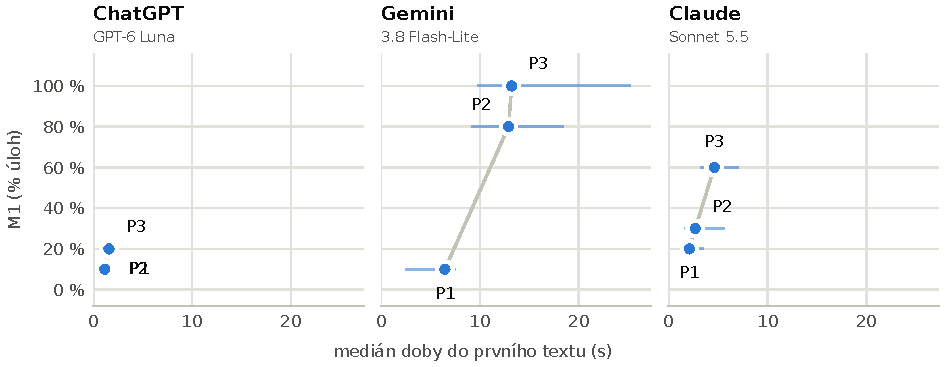
\includegraphics[width=\linewidth]{vystupy/graf_latence.pdf}
\caption{Kvalita a~rychlost: M1 proti mediánu doby do prvního textu odpovědi. Vodorovné úsečky jsou mezikvartilová rozpětí. Intervaly pro M1 jsou na obrázku~\ref{fig:m1}.}
\label{fig:latence}
\end{figure}

